\documentclass{article}

\usepackage[margin=1in]{geometry}   
\usepackage{graphicx}
\usepackage{caption}
\usepackage{subcaption}

\graphicspath{{diagrams/}}

\title{Overview TTC/Antenna Module}
\author{Bruno C. Messias}
\date{}

\begin{document}

\maketitle

\section{Requisitos Fundamentais}

\begin{itemize}
    \item Enviar dados em UHF e VHF
    \item Receber comandos da GroundStation para deploy
\end{itemize}

\begin{figure}[htbp]
    \centering
    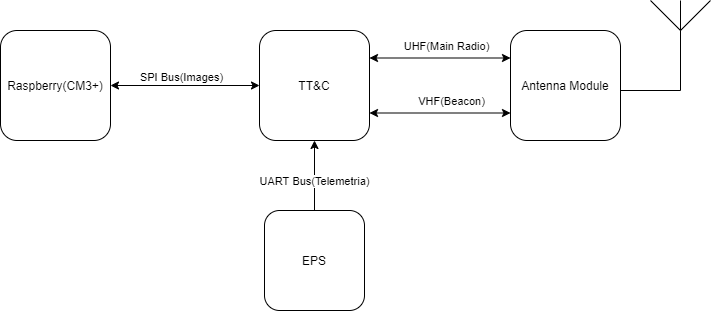
\includegraphics[scale=.5]{Datapath.png}
    \caption{Datapath Diagram}
    \label{datapath}
\end{figure}

\begin{figure}[htbp]
    \centering
    \includegraphics[scale=.5]{Control_signals.png}
    \caption{Control Signals Diagram}
    \label{signals}
\end{figure}

\begin{figure}[htbp]
    \centering
    \includegraphics[scale=.5]{Power_buses.png}
    \caption{Power Buses Diagram}
    \label{power}
\end{figure}


\end{document}